\chapter{Graphical Models}

\section{Latent Variable Models}

\subsection{Temporal Latent Variable Models}

We have a sequence of observations $\mathbf{x}_{\leq T}$, which extend over $T$ timesteps. Assume we also have a sequence of latent variables $\mathbf{z}_{\leq T}$. If we assume that time only moves in the forward direction, then with parameters $\theta$, we can write the joint probability of this model as

\begin{equation}
	p_\theta (\mathbf{x}_{\leq T}, \mathbf{z}_{\leq T}) = \prod_{t=1}^T p_\theta (\mathbf{x}_{t} | \mathbf{x}_{< t}, \mathbf{z}_{\leq t}) p_\theta (\mathbf{z}_{t} | \mathbf{x}_{< t}, \mathbf{z}_{< t}).
\end{equation}

\noindent The term $p_\theta (\mathbf{x}_{t} | \mathbf{x}_{< t}, \mathbf{z}_{\leq t})$ is the conditional likelihood or observation model, and the term $p_\theta (\mathbf{z}_{t} | \mathbf{x}_{< t}, \mathbf{z}_{< t})$ is the prior, transition, or dynamics model. The full graphical model is represented in figure \ref{fig: full_temporal_model}. The conditional dependencies show that the computation in this model grows exponentially with the sequence length $T$. Later, we will enforce stricter assumptions on the temporal dependencies to make computation tractable.

\begin{figure}[h]
    \centering
    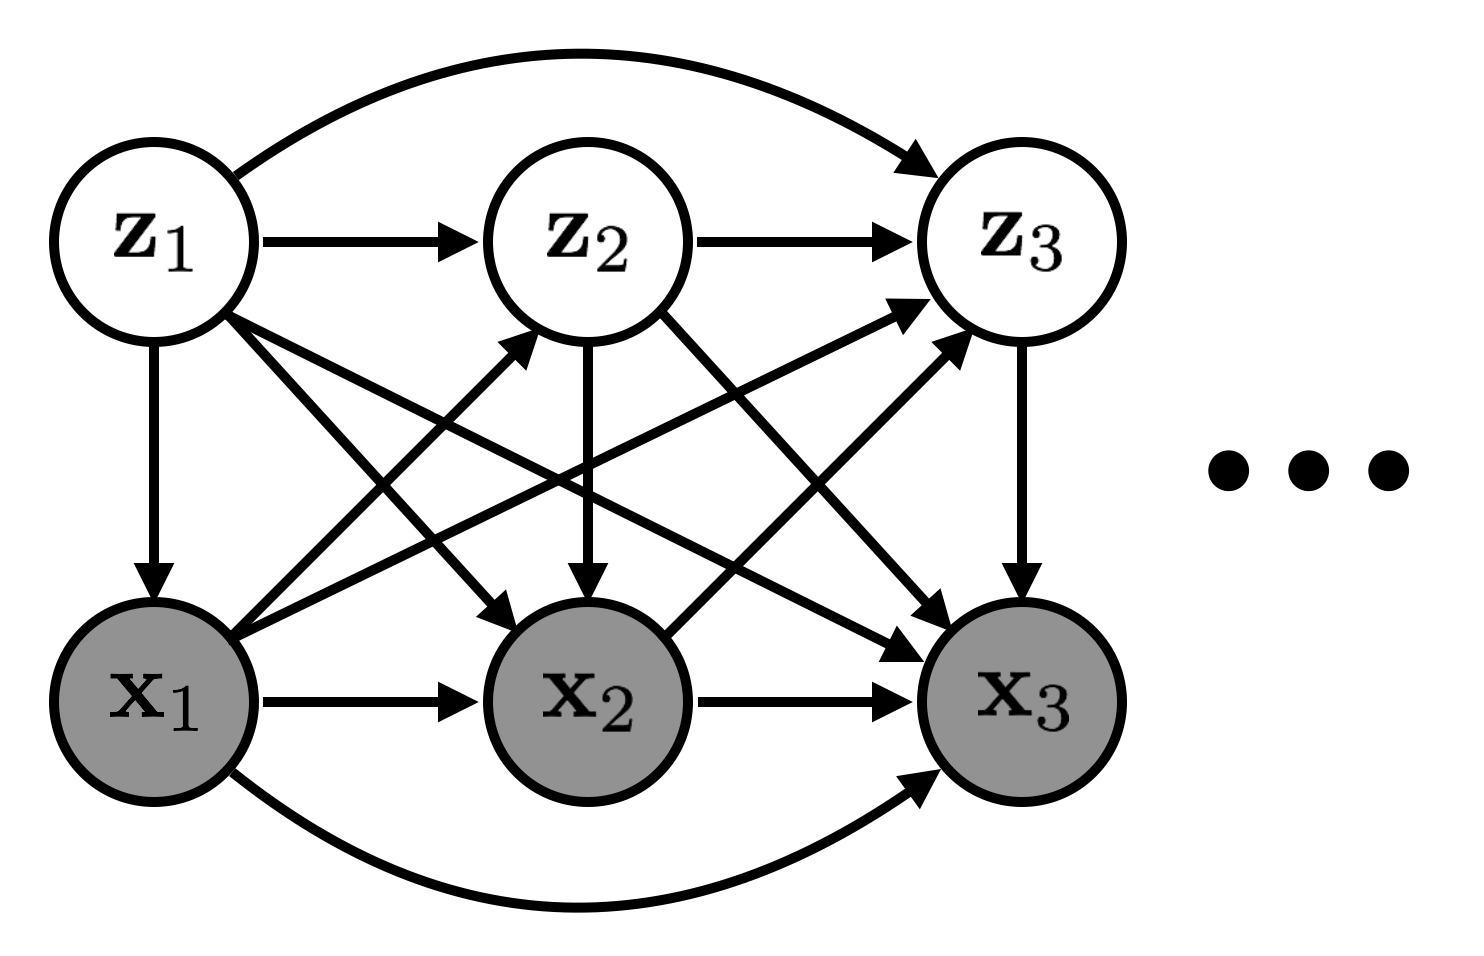
\includegraphics[width=.5\textwidth]{images/graphical_models/full_temporal_model.png}
    \caption{Simplified graphical model representation of temporal latent variable model with all connections present. Note that we're assuming the `arrow of time' points forward; variables can only affect other variables at the current time step or at future time steps. The parameters $\theta$ have been omitted for clarity.}
    \label{fig: full_temporal_model}
\end{figure}

To train or perform inference with this model, we need to compute $p_\theta (\mathbf{x}_{\leq T})$, which involves marginalizing over all states $\mathbf{z}_{\leq T}$:

\begin{equation}
	\log p_\theta (\mathbf{x}_{\leq T}) = \log \int p_\theta (\mathbf{x}_{\leq T}, \mathbf{z}_{\leq T}) d \mathbf{z}_{\leq T}
\end{equation}

\noindent Instead, we'll use an approximate posterior distribution, $q (\mathbf{z}_{\leq T} | \mathbf{x}_{\leq T})$, to compute a lower bound on this quantity:

\begin{equation}
	\log p_\theta (\mathbf{x}_{\leq T}) = \log \mathbb{E}_{q (\mathbf{z}_{\leq T} | \mathbf{x}_{\leq T})} \left[ \frac{p_\theta (\mathbf{x}_{\leq T}, \mathbf{z}_{\leq T})}{q (\mathbf{z}_{\leq T} | \mathbf{x}_{\leq T})} \right]
\end{equation}

\begin{equation}
	\log p_\theta (\mathbf{x}_{\leq T}) \geq \mathbb{E}_{q (\mathbf{z}_{\leq T} | \mathbf{x}_{\leq T})} \left[ p_\theta (\mathbf{x}_{\leq T}, \mathbf{z}_{\leq T}) - q (\mathbf{z}_{\leq T} | \mathbf{x}_{\leq T}) \right]
\end{equation}
